\documentclass[11pt,letterpaper]{article}
\usepackage{hyperref}
\usepackage[spanish]{babel}
\usepackage{multirow} 
\usepackage{multicol} 
\usepackage{subfig}
\usepackage{amsmath} % for \text{}
\usepackage{gensymb}
\usepackage{float}
\usepackage{mathrsfs} 
\usepackage{minted}
\usepackage{hyperref}

\usepackage[utf8]{inputenc}
% Control de color en tablas muy versátil.
\usepackage[table]{xcolor}
 % LaTeX


\title{Plantilla Informe}
  
% $Rev: 5 $
% PAQUETES %%%%%%%%%%%%%%%%%%%%%%%%%%%%%%%%%%%%%%%%%%%%%%%%%%%%%%%%%%%%%%%%%%%%
\usepackage{graphicx}
\usepackage{listings}
\usepackage{xcolor}
\usepackage{multicol}
\usepackage{anysize} %Permitir distintas medidas de margenes
\usepackage{framed}
\usepackage{fancyhdr}
\usepackage[spanish]{babel}
\usepackage[utf8]{inputenc}

\fancyhf{} 
\chead{ Proyecto de T\'itulo I \vspace{0.3cm}}
\lhead{
\includegraphics[scale=0.1]{Log.png}}
\rfoot{\thepage}

\renewcommand{\footrulewidth}{0.25pt}

\addtolength{\headheight}{1.4cm}

% CONFIGURACION DE LISTINGS %%%%%%%%%%%%%%%%%%%%%%%%%%%%%%%%%%%%%%%%%%%%%%%%%%%
\newcommand{\AddUserKeywords}[1]{\lstset{morekeywords=[2]{#1}}}
\newcommand{\CodeSize}[1]{\lstset{basicstyle=#1\ttfamily}}
\newcommand{\CommentColor}{\color{green!60!black}}
\newcommand{\StringColor}{\color{red!70!black}}
\newcommand{\UserKeywordsColor}{\color{cyan!50!black}}
\newcommand{\KeywordsColor}{\color{blue}}

\lstdefinelanguage{CSharp}
{
	basicstyle=\small\ttfamily,
	keywordstyle=\KeywordsColor\textbf,
	keywordstyle=[2]\UserKeywordsColor,
	keywordstyle=[3]\StringColor,
	tabsize=2,
	morekeywords={abstract, as, base, bool, break, byte, case, 
		catch, char, checked,class, const, continue, decimal, 
		default, delegate, do, double, else, enum, event, explicit,
		extern, false, finally, fixed, float, for, foreach, get, goto, 
		if, implicit, in, int, interface, internal, is, lock, long,
		namespace, new, null, object, operator, out, override, 
		params, partial, private, protected, public, readonly, ref, return, 
		sbyte, sealed, set, short, sizeof, stackalloc, static, string,
		struct, switch, this, throw, try, typeof, true, uint, ulong, 
		unchecked, unsafe, ushort, using, value, virtual, volatile,
		void, while, where},
	morekeywords=[2]{Main,Console,String},
	morekeywords=[3]{@}, 
	commentstyle=\CommentColor,
	stringstyle=\StringColor,
	sensitive=true,
	morecomment=[l]{//},
	morecomment=[s]{/*}{*/},
	morestring=[b]",
	showstringspaces=false,
	aboveskip=0pt, 
	belowskip=0pt,
	mathescape=true
}

% Set as the default languaje
\lstset{language=CSharp}

\newcommand{\inguandesheader}{
	% Header Facultad Ingenieria Uandes			
	
\includegraphics[scale=0.5]{uandes.pdf}\hspace*{\fill}
}

\newcommand{\evaluationtitle}[2]{
	% T\'itulo
	\begin{center}
	\vspace{1ex}\Large #1\\
	\vspace{1ex}\small #2
	\end{center}
}


\newenvironment{guideexercise}[3]{
	\noindent\textbf{#1}	
	\vspace{-0.3cm}
	\begin{framed}
		\noindent\textsl{Dificultad:} #2\\
		\textsl{Etiquetas:} #3\\	
				
}{
	\end{framed}
	\vspace{0.3cm}
}

\renewcommand{\baselinestretch}{1.5}

\pagestyle{fancy}
\begin{document}

%% COMIENZO PORTADA-----------------------------------------

\begin{titlepage}

\begin{center}

\includegraphics[scale=0.3]{Log.png}\\
% Incrementamos el interlineado:
\vspace{1.0cm} {\LARGE Hito II\\ Ingenier\'ia Civil Industrial UANDES\\  Proyecto de T\'itulo I} \\

\vspace{1.5cm} \LARGE{Por:\\ Ezequiel Ortiz Torres \\ Gu\'ia: \\ Sebasti\'an Cea}

\vspace{2.3cm}

\vspace{.5cm} \today

\end{center}
\end{titlepage}

 %%%% FIN PORTADA ------------------------------------------

\tableofcontents
\newpage


\section{Introducci\'on}

Un proyecto con características medioambientales, sociales y gubernamentales es un proyecto ESG por sus siglas en inglés (\textit{environmental, social \& governance}). Un estilo de inversión que se ve cada vez más expuesto ante la mirada de los fondos, cumpliendo un rol importante en las carteras, los administradores, el tipo de activo y el inversionista. Además, los proyectos se vuelven más sensibles a las tasas de interés.

Todo el estudio en el que está basado este experimento, modela la intención racional de un tomador de decisión (DM) siguiendo alguna de las cuatro funciones de costos. 
A continuación, se presenta una tabla sacada del trabajo de Dewan y Neligh (2020) donde se resumen las características de las funciones, junto con el comportamiento del desempeño. 


        \begin{figure}[h]
            \centering
            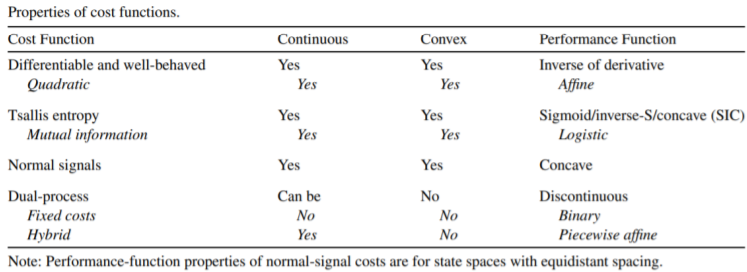
\includegraphics[scale=1]{Propiedades funciones de costo.png}
            \caption{Propiedades de funciones de Costos}
        \end{figure}


El comportamiento de un DM, al evaluar una determinada tarea como contar puntos, sujeta a un incentivo o premio por responder de forma correcta, se ajusta a una de estas funciones. Si bien cada función de costo genera una función de desempeño única, la recuperación de una función de costo a partir de una función de desempeño no es en general única. Sin embargo, se puede seleccionar una función de desempeño que mejor se ajuste en función del comportamiento observado de un DM, y este dato se puede usar para determinar cuál de un conjunto de clases plausibles de funciones de costo podría haber generado el comportamiento observado (Dewan y Neligh, 2020). 

De este modo, el experimento involucra una serie de tareas de percepción que serán descritas más adelante, que tienen una recompensa potencial. Los individuos deberán resolver estas tareas, sin saber los resultados hasta el final, y donde completar las pruebas de forma correcta, le atribuye un mayor grado de probabilidad para ganar el premio.

Solo para concluir, se utilizaron dos supuestos fundamentales. En primer lugar, se utilizaron 5 respuestas posibles y una correcta, y con esto se consideran las funciones de costos basadas en entropía, ya que no funcionaría en un mundo de selección binaria según señalan los autores Dean y Neligh (2020). Por otro lado, es importante tener niveles de incentivos distribuidos de forma aleatoria, al igual que la cantidad de puntos en cada prueba.





\subsection{Explicación simplificada del marco teórico.}

La investigación del trabajo nos indica que las decisiones de inversión se basan en incentivos y propone exponer como será el desarrollo de la toma de estas decisiones y la razón final por la cual sucede. Bajo este rápido y mínimo resumen, se lleva a cabo una compleja explicación en términos de funciones de costos, como la información disponible y el costo de adquirir nueva información, determinan la forma que adopta la toma de decisión frente a proyectos ESG.

Estas 4 funciones de costos se explican de forma simple de la siguiente manera:

\begin{enumerate}
    \item \textbf{Función de desempeño logístico:} o función de costos de información mutua, se explica como una validación a través de la información adquirida, es decir, la creencia a priori se condice con la creencia a posteriori. 
    \item \textbf{Función de desempeño sigmoidea, inversa o cóncava:} es una generalización de la función de costos de información mutua, conocida también como la función de costos de la entropía de Tsallis (cf.Caplin et al., 2019). Para este caso, la información no necesariamente va de la mano con lo que el tomador de decisión piensa previamente, sino más bien, puede diferir completamente y el resultado agrega mayor valor a la obtención del incentivo. 
    \item \textbf{Función de desempeño binaria:} con solo dos niveles de desempeño. Las decisiones son más directas, el comportamiento de la función tiene solo dos probabilidades de ocurrencia.
    \item \textbf{Función de desempeño cóncava:} que son costos para aumentar la precisión de esta información. En este caso, la información no es valiosa, y la decisión no se basa en la obtención de esta. 
    
\end{enumerate}

Un punto importante de todas estas funciones de costos es que la probabilidad de que DM decida correctamente aumenta en la medida que suben los incentivos, siendo una función continua y convexa. 

El marco teórico será explicado con un mayor detalle, a medida que avance la investigación.

\section{Experimentos}

En base al modelo original descrito y realizado por Dewan y Neligh (2020), se realizó un experimento alterno que luego será extrapolado al área de interés de la investigación. A continuación, se explica el experimento base y el experimento adaptado piloto junto con la presentación del código de programación con que se consiguió este resultado.

\subsection{Experimento Original}


El experimento de Dewan y Neligh (2020), se divide en dos partes, el conteo de puntos y el conteo de ángulos. En ambas experiencias, el DM está sometido a incentivos que podrá obtener si logra realizar una correcta participación. En principio, los sujetos completarán 200 tareas, cada una a un nivel de incentivo entero entre 1 y 100, inclusive. Primero se les mostrará al azar todas las tareas de 100 puntos o las 100 tareas de ángulo. Los bloques de tareas se equilibrarán por nivel de incentivo para garantizar
aproximadamente el mismo nivel de variación en los incentivos a lo largo del experimento. A
los sujetos se les mostrará primero cada uno de los 50 niveles de incentivos impares entre 1 y
100 en un orden aleatorio, y luego se les mostrará cada uno de los 50 niveles de incentivos
pares entre 1 y 100 en un orden aleatorio. Esto se repetirá (en un orden aleatorio diferente)
para las siguientes 100 tareas.
Las ganancias experimentales se determinarán de la siguiente manera. Una tarea de la primera mitad del experimento y una tarea de la segunda mitad del experimento se seleccionarán al azar para el pago. El nivel de incentivo de cada tarea seleccionada determinará la probabilidad de ganar uno de los dos premios monetarios. Por ejemplo, si la primera tarea seleccionada tenía un nivel de incentivo de 84 y se respondió correctamente,
y la segunda tarea seleccionada tenía un nivel de incentivo de 33 y se respondió incorrectamente, esto le daría al sujeto un 84 por ciento de probabilidad de ganar el primer premio, y un 0 por ciento de probabilidad de ganar el segundo premio. La determinación de las ganancias de
esta manera podrá asegurar que las ganancias esperadas sean lineales en el nivel de incentivos, lo que obviará la necesidad de obtener preferencias de riesgo. En otras palabras, esto asegura que, bajo el supuesto de la teoría de la utilidad esperada, podamos conocer las utilidades de los sujetos (excluyendo los costos de información, hasta una constante
multiplicativa). Así, la relación estimada entre desempeño y nivel de incentivo para cada
sujeto podría considerarse una estimación válida de su función de desempeño, sin necesidad de aplicar ninguna transformación adicional (Dewan y Neligh, 2020). 

\subsection{Explicación de la adaptación del experimento original}

Para este trabajo en particular, solo se utilizará en una primera instancia, un plan piloto que contempla el conteo de puntos durante 100 oportunidades, con incentivos que se mostrarán de 1 a 100, inclusive, de forma aleatoria, y que se irán sumando cada vez que un individuo responda de manera correcta.

En una primera parte, la pantalla muestra las instrucciones del juego, junto con el botón comenzar. Luego de presionar este botón, el juego comienza y aparece en pantalla durante 3 segundos el primer incentivo. Posteriormente, se despliega una imagen que contempla entre 38 y 42 puntos, inclusive, distribuidos de forma aleatorea, además de 5 botones con las alternativas, del 38 al 42, por lo que el DM podrá seleccionar la respuesta que crea correcta después de contar los puntos. 

A continuación, se muestra una secuencia de 4 imágenes que ejemplifican el juego:


\begin{figure}[h]
    \centering
        \subfloat[Pantalla de inicio]{
        \label{f:Pantalla de inicio}
            
\includegraphics[width=0.3\textwidth]{imagen 1.png}}
        \subfloat[insentivo]{
        \label{f:Insentivo}
            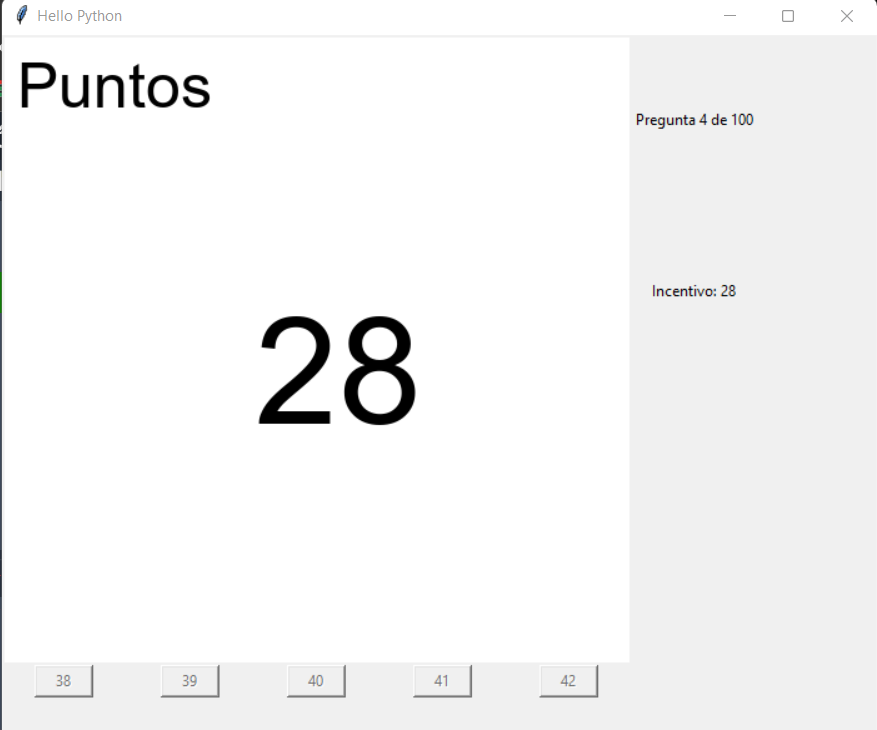
\includegraphics[width=0.3\textwidth]{imagen 2.png}}
\end{figure}
\begin{figure}[h]
    \centering
        \subfloat[Puntos distribuidos]{
        \label{f:Puntos distribuidos}
            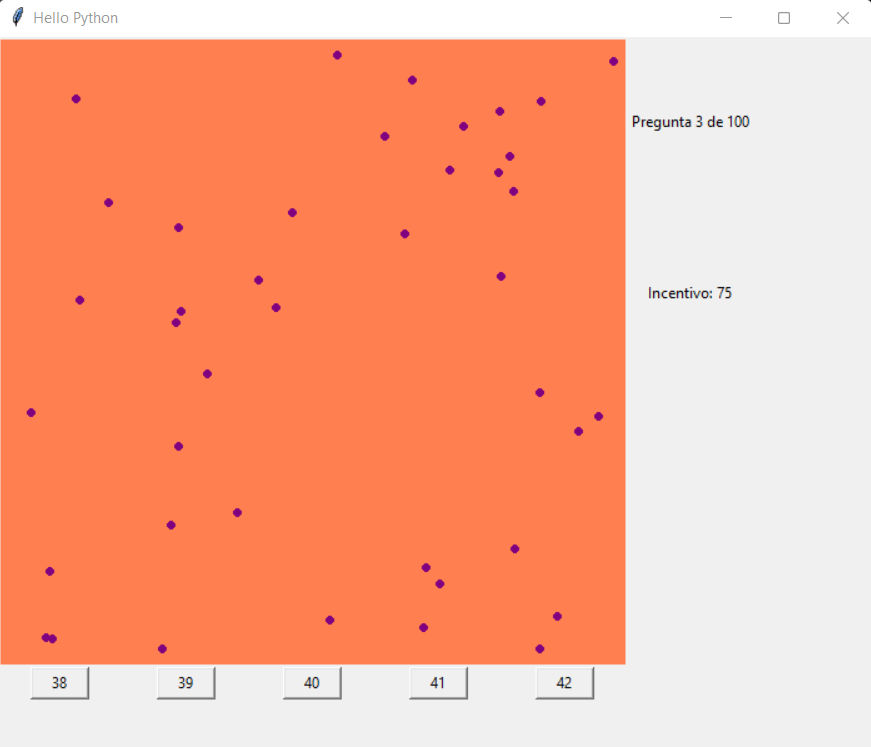
\includegraphics[width=0.3\textwidth]{imagen 3.png}}
        \subfloat[Resumen Final]{
        \label{f:Resumen Final}
            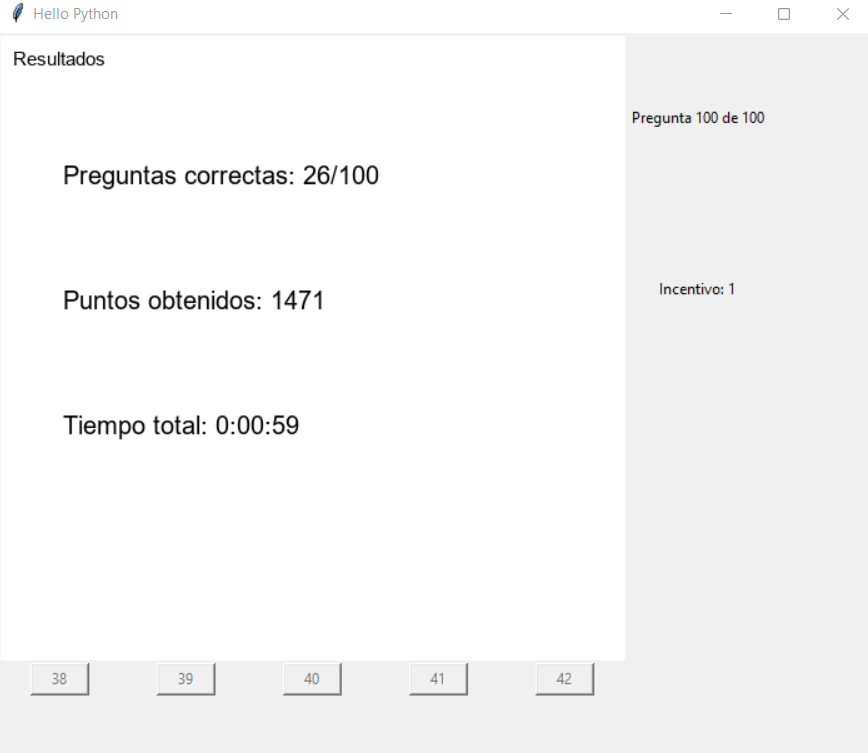
\includegraphics[width=0.3\textwidth]{imagen 4.png}}
    \caption{Adaptación experimento Dean y Neligh (2020)}
\end{figure}

Al finalizar, se entregan en la pantalla un resumen de la experiencia, con el total de respuestas correctas, el número que suman los incentivos percibidos por responder bien, y el tiempo que tardó en responder los 100 conteos.

\subsection{Código del experimento piloto en Python}

El experimento piloto se realizó utilizando el lenguaje Python de programación. Son 157 líneas de código (Anexo 1), y se utilizaron las librerías \textit{tkinter} y \textit{Pillow}, que fueron necesarias para generar las imágenes.

Podemos dividir el código en 4 partes claves.

\begin{enumerate}

\item En la primera parte del código, se crea la función que generará las coordenadas aleatorias de los puntos, con las restricciones para que no se sobrepongan nunca.
\item Luego, se definen funciones para generar la distribución de los puntos, las instrucciones, los incentivos, su distribución y la pantalla final de resumen.
\item El siguiente paso fue configurar los botones que contienen las respuestas correctas de cada experiencia de conteo. Estos, se van deshabilitando cada vez que se muestra un incentivo. Contienen dos contadores, uno para el número de preguntas que se detendrá al llegar a 100, y otro para sumar los puntos ganados con cada respuesta correcta. 
\item El módulo \textit{draw} se utiliza para generar las imágenes que va a contener el juego, como las instrucciones, incentivos y los puntos junto con el resumen final. Si bien definimos funciones que generan estas distribuciones, con este módulo estas son plasmadas en imágenes.
\item Por último, está la configuración del texto que están por los costados de la pantalla principal como imágenes, junto con los botones de la parte de abajo. 
\end{enumerate}
Las siguientes imágenes, muestran el código de acuerdo con cada explicación de este punto.

\begin{figure}[h]
    \centering
        \subfloat[Coordenadas puntos]{
        \label{f:Coordenadas puntos}
            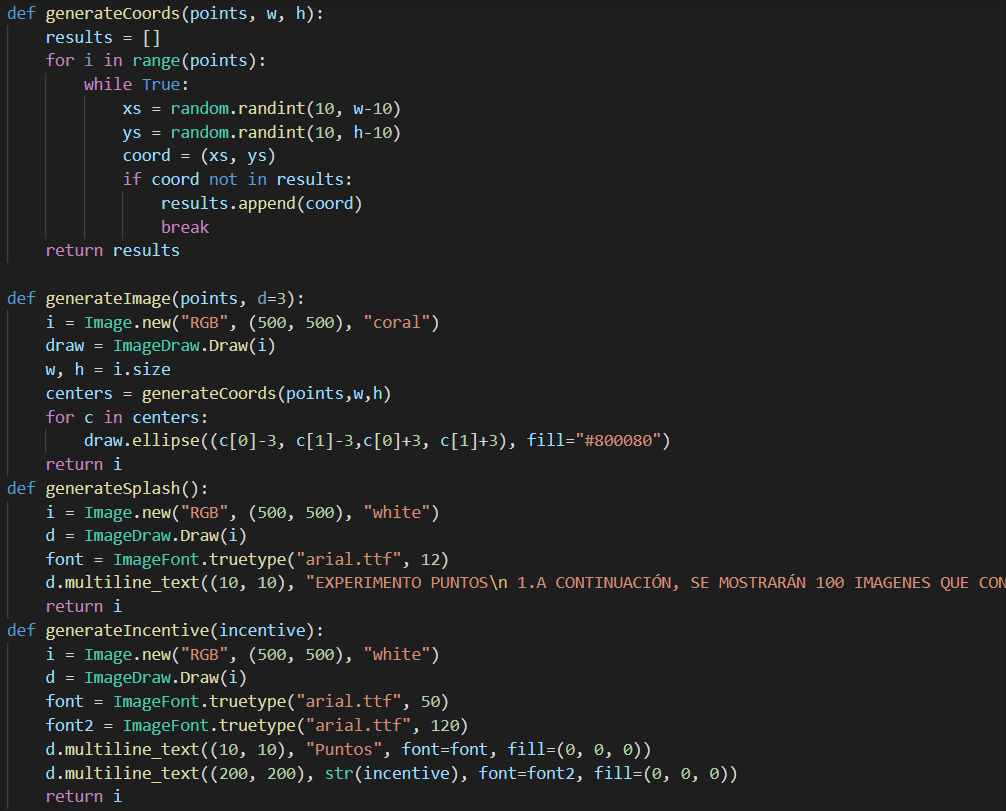
\includegraphics[width=0.45\textwidth]{codigo .png}}
        \subfloat[Definición de funciones]{
        \label{f:Definición de funciones}
            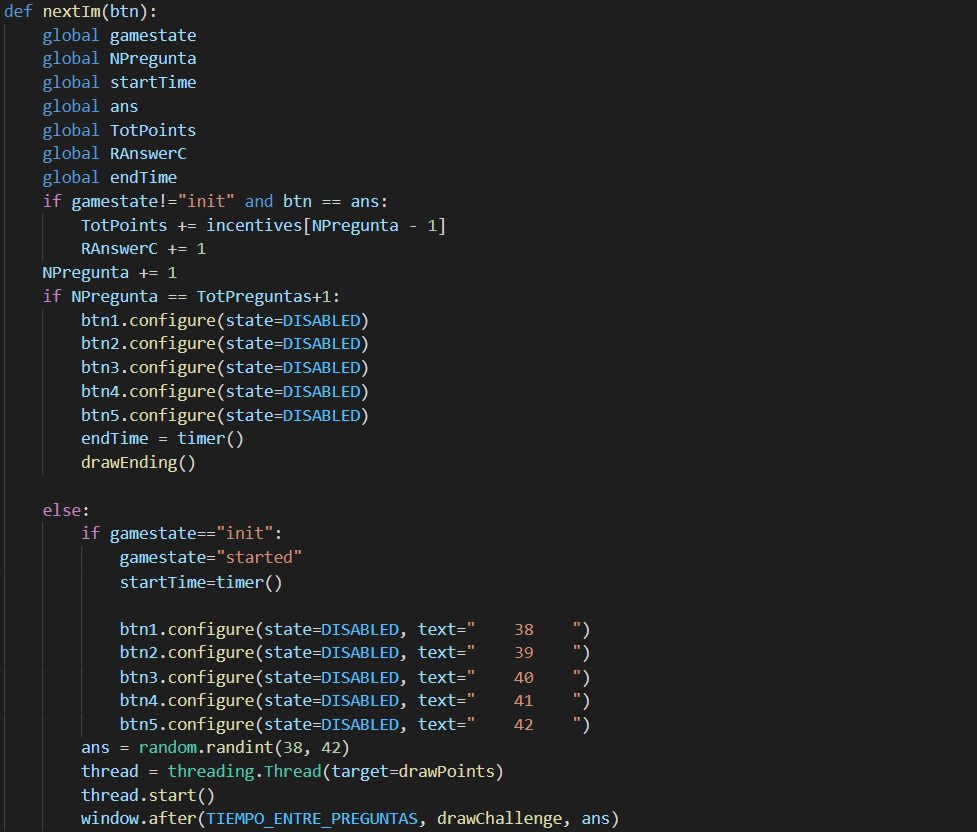
\includegraphics[width=0.45\textwidth]{codigo 2.png}}
\end{figure}
\begin{figure}[h]
    \centering
        \subfloat[Modulo draw]{
        \label{f:Modulo draw}
            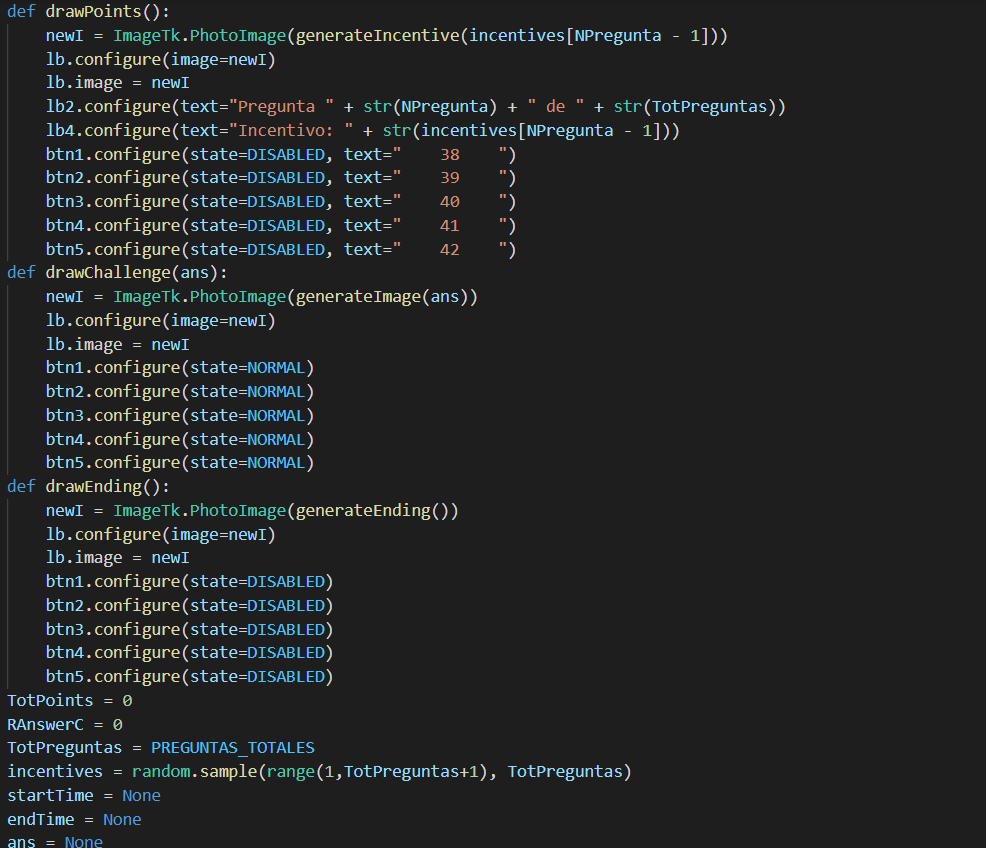
\includegraphics[width=0.45\textwidth]{codigo 3.png}}
        \subfloat[Otras configuracionesl]{
        \label{f:Resumen Final}
            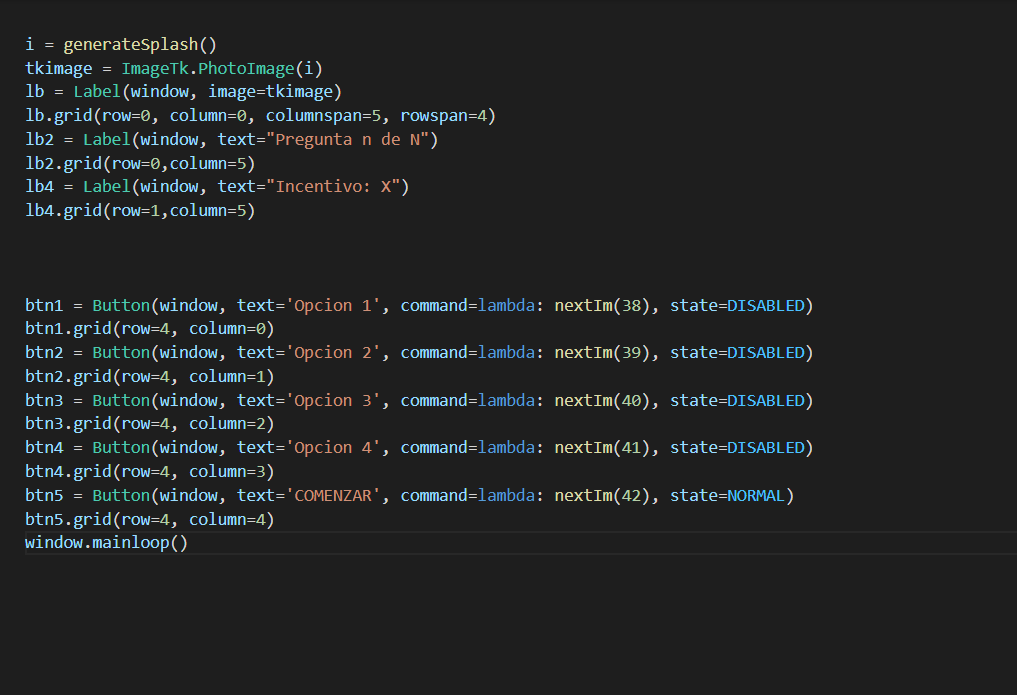
\includegraphics[width=0.5\textwidth]{codigo 4.png}}
    \caption{Código experimento piloto}
\end{figure}






\newpage
\section{El Ecosistema ESG}

Se llamará Ecosistema ESG a todo lo que envuelve la toma de decisiones con respecto a los proyectos sustentables. Los actores tienen distintos niveles de importancia en esta área, y cumplen roles que son detallados a continuación. 

En primer lugar, los criterios ESG tienen origen en los años 60, posterior a la guerra de vietnam, cuando los universitarios estadounidenses se vieron envueltos en protestas exigiéndoles a las universidades no invertir en instrumentos militares según señala la página del Banco Santander (2020), en su artículo sobre la definición de estos criterios. 

Además, los 3 factores en que se fundamentan estos criterios son los siguientes:

\begin{enumerate}

\item El factor ambiental (E), para tomar decisiones en función de cómo afectan las actividades de las empresas en el medio ambiente.
\item El factor social (S), para tener en cuenta la repercusión que tienen en la comunidad las actividades desempeñadas por la compañía, por ejemplo, en términos de diversidad, derechos humanos o cuidados sanitarios.
\item El factor de gobierno (G), que estudia el impacto que tienen los propios accionistas y la administración, y se basa en cuestiones como la estructura de los consejos de administración, los derechos de los accionistas o la transparencia, entre otros.

\end{enumerate}

\subsection{Descripción del Ecosistema:}

\subsection{Fondos de Inversión:}

Son los tomadores de decisiones por definición. Como entidad, funcionan a través de mediciones llevadas a cabo por instrumentos de análisis tanto humanos como a nivel de software. Esto determina un orden jerárquico entre las primeras evaluaciones hasta la decisión final de inversión.

\subsection{Gobierno:}

El gobierno toma parte importante en el ecosistema ESG. El poder legislativo a través de leyes y regulaciones dicta argumentos importantes para que las empresas guíen sus actividades en pos de características sustentables. Un ejemplo de esto son la ley de fomento al reciclaje, contenida en la ley N° 20.920 (Biblioteca del Congreso Nacional, 2016) o en el plan de Acción Nacional de Cambio Climático (PANCC 2017-2022), que contribuye a uno de los más importantes objetivos del desarrollo sustentable: aportar a la reducción del calentamiento global. 

Otro punto importante es la CORFO (Corporación de fomento a la producción) que constantemente está llamando a participar por fondos, como capital semilla entre otros, con el requisito de tener características sustentables dentro de los proyectos. 

\subsection{Proyectos y empresas:}
En este nivel se encuentran todos los emprendedores, las pymes y también los negocios medianos y grandes (a través de la venta de bonos verdes, por ejemplo), quienes presentan una oportunidad a los fondos, desencadenando todo lo anterior. Sin las ideas sustentables no existe análisis ni ecosistema.

Para describir mejor lo anterior, se presenta un esquema de elaboración propia con el objetivo de explicar a priori, lo que se espera encontrar en este ecosistema, y postula la hipótesis de que todo instrumento de medición será observado con ojos muy distintos dependiendo del nivel y el rol desempeñado, y buscará establecer recomendaciones para los distintos actores involucrados.

\begin{itemize}
    \item Esquema Ecosistema ESG
        \begin{figure}[h]
            \centering
            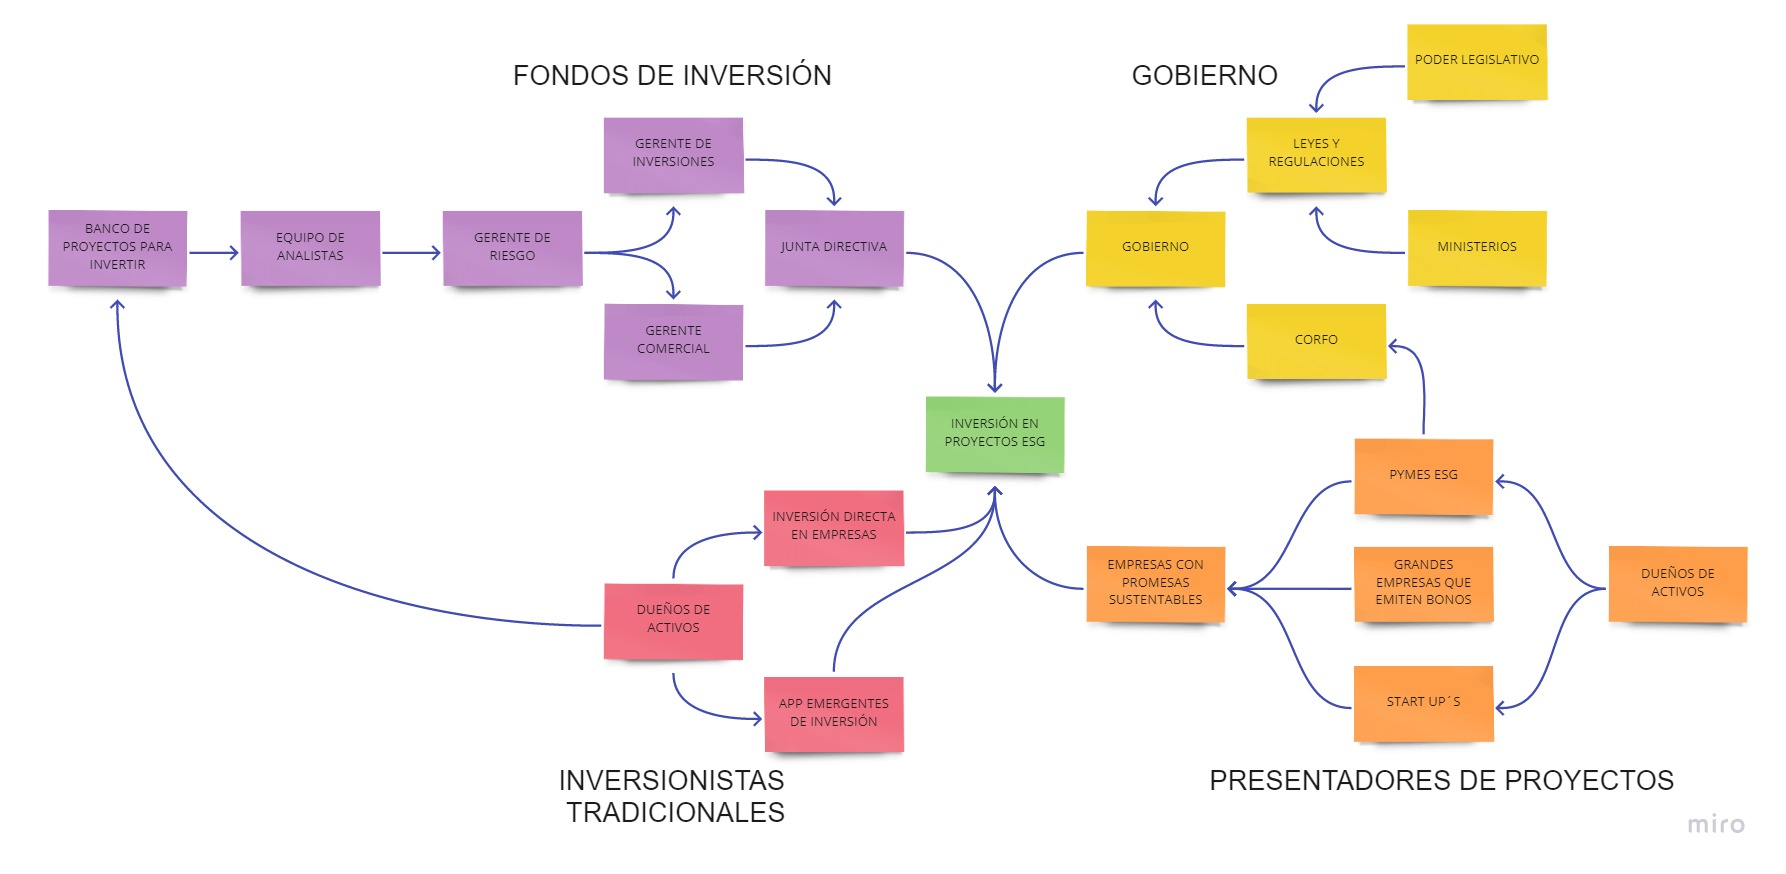
\includegraphics[scale=0.2]{Concept Map - Frame 1.jpg}
            \caption{Ecosistema ESG}
        \end{figure}
\end{itemize}

En este esquema, los actores pueden ser los inversionistas o dueños de activos que trabajan su capital de distintas formas. En rojo aparecen los inversionistas más "tradicionales", que depositan su dinero en aplicaciones modernas como Fintual o Racional. También, invierten a través de fondos de inversión, señalados en color morado, las cuales realizan contribuciones y compras de bonos en proyectos ESG.

En amarillo está el gobierno, que además de regular, también invierte con criterios ESG, y tiene instrumentos como CORFO. 

Finalmente, en Naranjo aparecen las empresas como tal, que tienen las ideas sustentables y que se desempeñan gracias a las inversiones.



\section{Entrevistas}

Según Belsom, Ahour, et all (2021), la interacción entre los dueños de activos y quienes los administran no siempre se condice, además de estar cada vez más presente las expectativas de las políticas ESG.

Por un lado, un incentivo para adoptar características ESG concuerda con los beneficios de la tasa de interés y puede depender del área geográfica donde se encuentran los actores, junto a las leyes y políticas públicas a las que se deben adecuar. 

Esta primera etapa de la investigación se centrará en los incentivos. La forma e importancia con que llegan los incentivos a todos quienes se involucran en la inversión de un proyecto es relevante para la toma de decisión. De este modo, las preguntas son variadas y diferentes dependiendo de las características del estatus del individuo.

Por el momento, las entrevistas están a la espera de contactar con éxito a interesados en participar del proyecto. Se hizo un trello que dividió a los posibles participantes en distintas etapas y niveles.
Actualmente en chile, la mayor parte de los fondos de inversión o empresas de distintos rubros tienen un área sostenible, dentro de las que destacan: FIS AMERIS, FEN VENTURES, SEMBRADOR AGRICULTURAL INVESTIMENTS, SEDAMERIK INVERSIÓN DE IMPACTO, LUMNI, QUES CAPITAL, START UP CHILE, CORFO, GSG, BANCO BICE, LARRAÍN VIAL, CAPITALIA, FUNDACIÓN NOCEDAL, entre otros. El objetivo para poder trabajar en el experimento final de la investigación es lograr conseguir una entrevista con al menos un integrante de cada empresa antes del comienzo del próximo año académico.
Las etapas en que ha sido dividido el proceso de entrevistas son tres. En un inicio, se tiene el listado de empresas y algunos candidatos. El siguiente paso es conseguir con las entrevistas que las personas accedan a participar de la experiencia en sí, para luego recopilar los datos de las pruebas realizadas. 

\subsection{Preguntas:}

Estas son algunas de las preguntas que se podrán realizar. Para poder encausar de mejor forma la información, se dividió en tres secciones según el tipo de entrevistados. En los primeros dos grupos, están quienes deben aprobar y argumentar frente a un proyecto en los que pueden invertir, y, por otro lado, se encuentran las personas que deben vender los proyectos frente a los inversionistas. Además, es consecuente decir que solo los dos primeros grupos podrán realizar la prueba y su experiencia nos servirá como data, y el tercer grupo solo nos brindará \textit{feedback} para poder realizar un experimento con todos los actores de un ecosistema.

De esta forma, las preguntas para los directores y gerentes de alto nivel serán las siguientes:

\begin{enumerate}
    \item ¿Qué entiende por Sustentabilidad? Es importante conocer las distintas respuestas, en este caso de forma muy general, con respecto al centro de la investigación.
    \item ¿Los retornos que espera en un proyecto sustentable son siempre de carácter monetario? Para este punto, conocer si los DM están esperando algo más allá de los beneficios monetarios comúnmente utilizados para evaluar cualquier proyecto. 
    \item ¿Qué tanto puede llegar a influir las características ESG en cuanto a los retornos por sobre las ganancias monetarias? Para unirla con la pregunta anterior, se espera que la mayoría indique que espera retornos en otros ámbitos.
    \item ¿Considera suficiente con cumplir planes regulatorios, o busca ir más allá en las apuestas con proyectos conscientes?
    \item ¿Cómo enfrentar la crisis del calentamiento global con sus puestos de poder ante decisiones tan trascendentales?
    
    
\vspace{1cm}    

Por otro lado, a los analistas de datos que están encargados de generar reportes y KPI sobre los proyectos:
    
    \item ¿Qué canales de información utilizan para medir características ESG?
    
    \item ¿Cuáles son las más influyentes?

    \item ¿Cree que las políticas de estado están siendo suficientes, o espera que mejoren y aumenten en la línea sustentable?
    
    
\vspace{1cm}


Por último, todas aquellos que buscan financiar sus proyectos a través de los fondos y otro tipo de instituciones (como fundaciones):

    \item ¿Es la educación el proyecto más sustentable por el cuál las grandes empresas junto con el gobierno deberían apostar?
    \item ¿Piensa que una buena alternativa para inversiones ESG es basarse siempre en explicar bien los retornos monetarios, e incluirlos como eje principal para su desarrollo?
    \item Es la promesa de sustentabilidad el eje central de los proyectos modernos.
    \item consideraría que es un valor agregado la sustentabilidad, o es más una responsabilidad y obligación.
    
Estas preguntas desarrolladas de forma preliminar están sujetas a cambio, pudiendo ser más, y dirigidas a más de un nivel.

\section{Propuesta Experimento en desarrollo}

Hay varios caminos que se pueden tomar para extrapolar el experimento base o piloto, a algo más complejo en términos de recibir información. De forma preliminar, dependiendo de los datos recopilados de las entrevistas y de no alejarse del experimento base (conteo de puntos).
Imaginemos un plano cartesiano, que en cada dirección conforme avanza en los ejes demuestra el aumento de un indicador (x,y) = (retorno, contaminación), y que además los puntos aparezcan distribuidos de forma aleatoria por debajo de la curva de costos. 

\section{Conclusiones}

En esta primera parte se estudió el experimento de Dewan y Neligh (2019) en detalle, se explicó de forma simplificada el marco teórico y se conectó directamente con la investigación en inversiones sostenibles. 

Se logró replicar en parte el experimento de puntos con el objetivo de poder extrapolar esta experiencia hacia un futuro experimento con mayor complejidad en las mediciones, pruebas a realizar, y los datos que se puedan recopilar. 
El compromiso de los trabajos futuros es encausar las ideas sobre encuestas y entrevistas para poder obtener la mayor cantidad de recursos sobre sustentabilidad por parte de los mismos actores del ecosistema descrito, y con eso, decidir cual será la mejor versión del nuevo experimento.

\newpage

\section{Bibliografía}

- Sostenibilidad | Banco Santander Chile [en línea]. (sin fecha). ¿Qué podemos hacer por ti hoy? | Banco Santander. [Consultado el 19 de noviembre de 2021]. Disponible en:

https://banco.santander.cl/nuestro-banco/sostenibilidad

- Dewan, A. y Neligh, N., (2020). Estimating information cost functions in models of rational inattention. Journal of Economic Theory [en línea]. 187, 105011. [Consultado el 19 de noviembre de 2021]. Disponible en: doi: 10.1016/j.jet.2020.105011

- Raglianti Borbolla, G., (2018). Aplicación de principios de democracia ambiental en la Ley N° 20.920, marco para la gestión de residuos, la Responsabilidad Extendida del Productor y fomento al reciclaje. Revista de Derecho Ambiental [en línea]. (10), 69. [Consultado el 19 de noviembre de 2021]. Disponible en: doi: 10.5354/0719-4633.2018.51983

- Plan de Acción Nacional de Cambio Climático 2017-2022 (PANCC-II) [en línea]. (sin fecha). mma.gob.cl. [Consultado el 19 de noviembre de 2021]. Disponible en: https://mma.gob.cl/cambio-climatico/plan-de-accion-nacional-de-cambio-climatico-2017-2022-pancc-ii/

- Embedding ESG factors in investment mandates [en línea]. (sin fecha). PRI. [Consultado el 19 de noviembre de 2021]. Disponible en: https://www.unpri.org/mandate-requirements-and-rfps/embedding-esg-factors-in-investment-mandates/8563.article

\newpage


Nota (escala 1 a 7): 
\vspace{3cm}
Observaciones



\centering Firma Guía



    
\end{enumerate}





\newpage

\section{Anexos}

\subsection{Anexo 1}











































%ejemplo Plantilla



\end{document}
